\documentclass[a4paper,twoside, openright,12pt]{report}
\usepackage{psfrag,amsbsy,graphics,float}
\usepackage[dvips]{graphicx, color}
\usepackage[latin1]{inputenc}
\usepackage{verbatim} 
\usepackage{appendix}

% MY CHANGE
%\usepackage[bookmarksnumbered=true]{hyperref} 

\usepackage[bookmarks=true,colorlinks=true,       % false: boxed links; true: colored links
    linkcolor=black,          % color of internal links
    citecolor=black,        % color of links to bibliography
    filecolor=black,      % color of file links
    urlcolor=black           % color of external links
]{hyperref}
 

%%% Stand 14.09.2007
%%% erstellt von Marion Sobotka
%%% marion.sobotka@tum.de
%%% last changes: 14.01.09


%_______Kopf- und Fu�zeile_______________________________________________________
\usepackage{fancyhdr}
\pagestyle{fancy}
%um Kopf- und Fu�zeile bei chapter-Seiten zu reaktivieren
\newcommand{\helv}{%
   \fontfamily{phv}\fontseries{a}\fontsize{9}{11}\selectfont}
\fancypagestyle{plain}{	
	\fancyfoot{}% keine Fu�zeile
	\fancyhead[RE]{\helv\leftmark}% Rechts auf geraden Seiten=innen; in \leftmark stehen \chapters
	\fancyhead[LO]{\helv\rightmark}% Links auf ungeraden Seiten=au�en;in \rightmark stehen \sections
	\fancyhead[RO,LE]{\thepage}}%Rechts auf ungeraden und links auf geraden Seiten
%Kopf- und Fu�zeile f�r alle anderen Seiten
\fancyfoot{}
\fancyhead[RE]{\helv\leftmark}
\fancyhead[LO]{\helv\rightmark}%alt:\fancyhead[LO]{\itshape\rightmark}
\fancyhead[RO,LE]{\thepage}
%________________________________________________________________________________


%_Definieren der R�nder und L�ngen__________
\setlength{\textwidth}{15cm}
\setlength{\textheight}{22cm}
\setlength{\evensidemargin}{-2mm}
\setlength{\oddsidemargin}{11mm}
\setlength{\headwidth}{15cm}
\setlength{\topmargin}{10mm}
\setlength{\parindent}{0pt} % Kein Einr�cken beim Absatz!!
%___________________________________________


%_______Titelseite__________________________________________
\begin{document}
\pagestyle{empty}
\enlargethispage{4.5cm} %Damit das Titelbild weit genug unten ist!
\begin{center}
\phantom{u}
\vspace{0.5cm}
\Huge{\sc Numerical Test Rig for Large-Scale and Interconnected Dynamical
Systems}\\
\vspace{1.5cm}
                                 \large{submitted\\
				  Project Laboratory\\
				  Networked and Cooperative Control\\
			  %DIPLOMARBEIT\\%/STUDIENARBEIT/MASTERRBEIT/BACHELORARBEIT\\ 
                               %            von\\
                              %  \large{Zwischenbericht zur\\
			%DIPLOMARBEIT/STUDIENARBEIT/MASTERARBEIT/
					   % BACHELORARBEIT\\ 
					   by         

						
					\begin{tabular}{c c}
					    \vspace{0.4cm} & \vspace{0.4cm} \\
					 cand. ing. Francisco Llobet& cand. ing. Jose Rivera  \\
						\vspace{0.5cm} & \vspace{0.5cm}\\
					born on December 18, 1986 & born on December 18, 1986\\
					resident: & resident:\\
					Amalienstr. 87& Amalienstr. 87\\
					80799 M\"{u}nchen & 80799 M\"{u}nchen  
					\end{tabular}

					                           
					%Tel.: +49\,176\,233\,14721\\
					\vspace{1.5cm}
					Institute of\\
					Automatic Control Engineering\\
					Technische Universit\"{a}t M\"{u}nchen\\
					\vspace{0.3cm}
					Univ.-Prof. Dr.-Ing./Univ. Tokio Martin Buss\\
                                        Univ.-Prof. Dr.-Ing. Sandra Hirche}
\end{center}
\vspace{2.5cm}
\begin{tabular}{ll}
Supervisor: & F. Deroo, S. Erhart, A. Gusrialdi, H. Mangesius  \\
Beginn: & 09.05.2011  \\
Submitted &  04.07.2011 \\
\end{tabular}
%____________________________________________________________

\newpage

%_______Abstract_____________________________________________
\topmargin5mm
\textheight220mm
\pagenumbering{arabic}
\phantom{u}
\begin{abstract}
The goal of this project was to develop a test rig for large-scale and interconnected dynamical systems. The result is
MTIDS or Matlab Toolbox for Interconnected Dynamical Systems, which is a mash-up that wraps different toolboxes used for graph analysis and 
dynamic systems simulation together. MTIDS allows the definition and analysis of graphs, where each node has a specific dynamic assign to it. 
The template based design of nodes' dynamics allows great flexibility for the creation of complex interconnected dynamical systems with the 
possibility of implementing clusters/layers. MTIDS is an open-source project under the GNU GPL v2 license. This document presents a general desciption 
of MTIDS and intructions for its use.    
%\vspace{2cm}
% \begin{center}
% \normalsize \textbf{Zusammenfassung}\\
% \end{center}
% Dieser Hauptseminar besch\"{a}ftigt sich mit der Methode der getriggerten Optimierung. Dabei wird besonderen Focus auf die m\"{o}glichen Anwendungen f\"{u}r Energiesystemen gesetzt.
% Als erstes wird eine Analyse der Methode in ihre genaralisierte Form f\"{u}r das NUM (Netzwerk Nutzen Maximirung) Problem durchgef\"{u}hrt. Als zweites wird ihre Anwendung an das OPF (Optimale Leistungsfluss) in Energienetzen evaluiert. Als letztes werden
% verbesserungs Vorschl\"{a}gen und weitere Anweundungen in Energiesystemen diskutiert.  
\end{abstract}
%____________________________________________________________

\newpage

%_______Widmung_______________________________________________
\phantom{u}
\phantom{1}\vspace{6cm}
\begin{center}
%Hier die Widmung oder leer lassen
\end{center}
%_____________________________________________________________



\pagestyle{fancy}

%_________Inhaltsverzeichnis__________________________
\tableofcontents 
%_____________________________________________________




%_________Einleitung__________________________________
\chapter{Introduction} \label{chapter1}

In this first Chapter the motivation behind the MTIDS project is explained and the project's goal and framework is presented.

\section{Motivaion}
Large-scale interconnected dynamical system are everywhere: biological systems, power and water systems, the brain neurons, 
social interaction networks, economic markets, etc. In a cononical form all of this systems can be thought as a bunch of nodes with local dynamics 
that interact with each other, e.g. a graph. Different topologies of the graph, may lead to different behavior. An example of various 
large scale interconnected systems can be seen in Figure \ref{largePic}. 


\begin{figure}[htb]
\centering
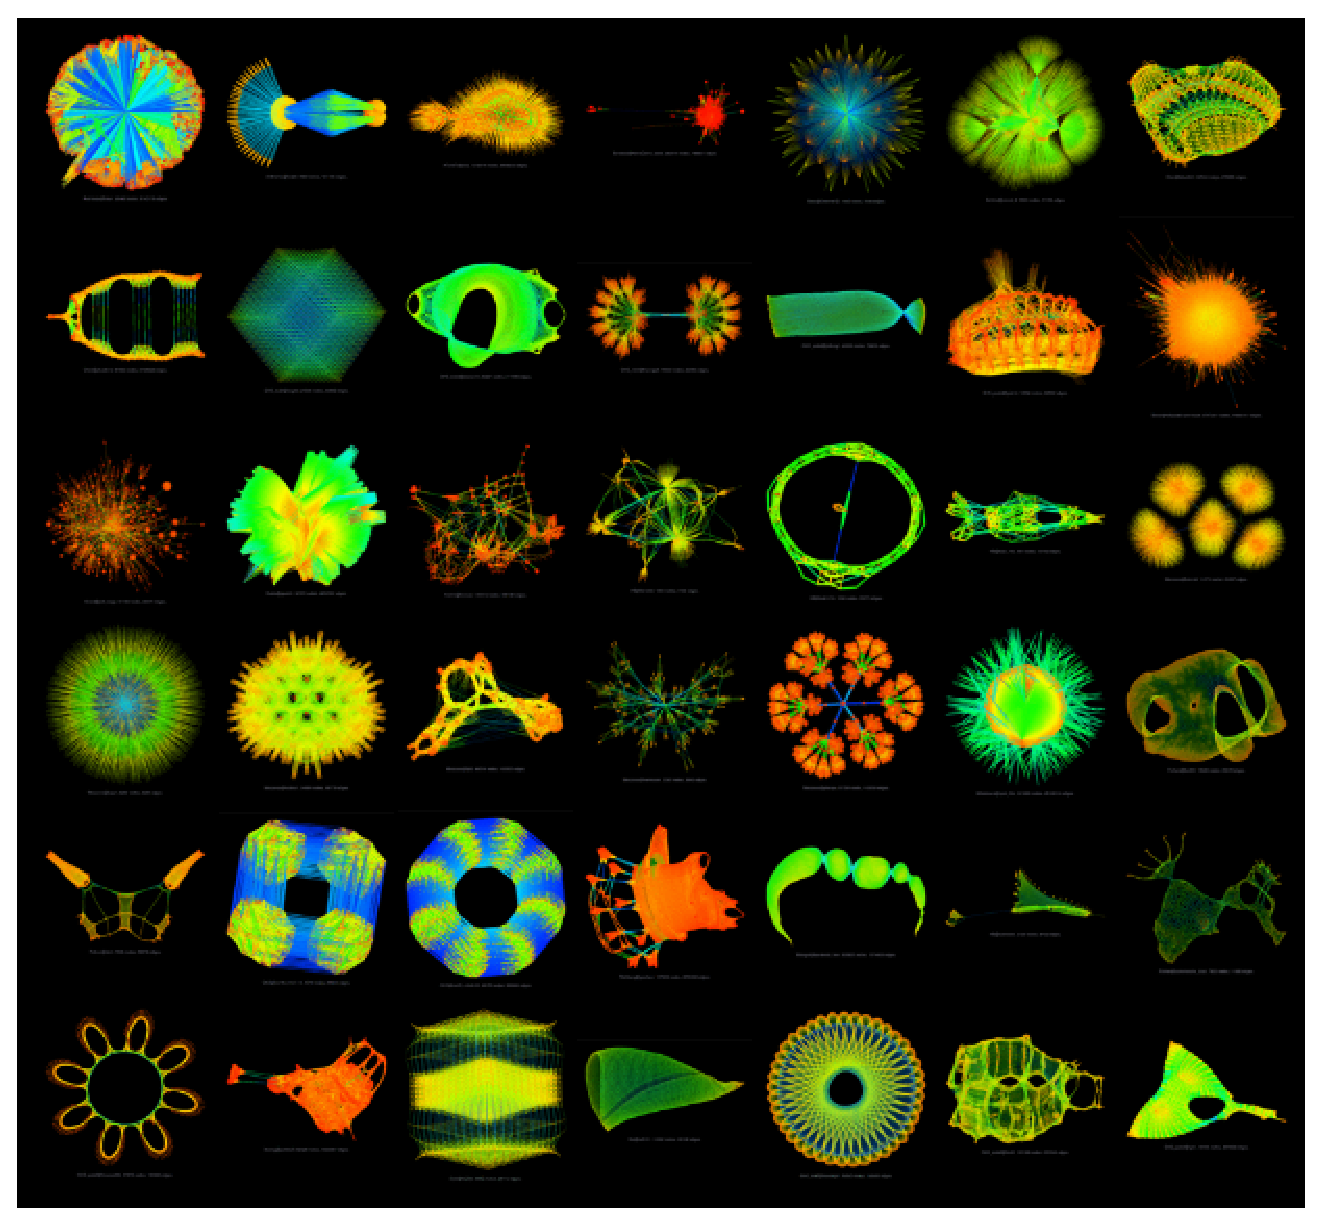
\includegraphics[width=0.5\textwidth]{pics/complex.eps}
\caption[Example of large-scale systems]{Visualization of various large scale systems using the sfdp algorithm $\copyright$ Dr. Yifan Hu of AT\&T Labs}
\label{largePic}
\end{figure}

There are many tools available for the analysis of interconnected dynamical systems, for example in power systems you have PSSE and Power Factory. However,
this simulation programs are normally very system specific and in most cases it takes a long time to learn how to use them correctly. 
The difficulties are specially noticed while
testing control concepts, where small changes on the topology of the grid or control concept could lead to a painful redesign of your simulation set up. 
You may actually end up spending the most of your time in the implementation of a simulation. A more general and 
easy to use solution for the simulation of interconnected dynamical systems is needed.




\section{Idea and Goal}

\textbf{MTIDS} (Matlab Toolbox for Interconnected Dynamical Systems) is a project that aims to design an easy 
to use and flexible toolbox to make the simulation of large scale dynamical systems easier for students and researchers. 
The \textbf{goal} is to produce a mash-up that wraps different toolboxes used for graph analysis and 
dynamic systems simulation together into a framework.  


\begin{figure}[htb]
\centering
\includegraphics[width=0.5\textwidth]{pics/mtidsstructure.eps}
\caption[MTIDS idea]{MTIDS: Matlab Toolbox for Interconnected Dynamical Systems}
\label{mtidsFig}
\end{figure}

As we can see in Figure \ref{mtidsFig} MTIDS runs in the MATLAB enviroment and is basically a GUI that allows the interaction of tools used in graph theory 
and control theory.  For graph theory we use Matgraph a toolbox design by Prof. Scheinerman of the John Hopkins University and for dynamical simulations
we use Simulink. 

\section{Framework}

The current framework of MTID is made out of three basic composnents. A GUI (\textbf{mtids.m}) an export to simulink function (\textbf{exportSimulink.m}) and
an inport from Simulink function (\textbf{importSimulink.m}).\\

 

\begin{figure}[htb]
\centering
\includegraphics[width=0.5\textwidth]{pics/uml.eps}
\caption[MTIDS components]{MTIDS: Components diagram}
\label{componentsFig}
\end{figure}

In Figure \ref{componentsFig} we can see that the most important component is the user, specially its head. The better you are at producing templates
and interacting with matlab and simulation the more functional MTIDS is going to be for you.
In a nutshell MTIDS works as fallows:
\begin{itemize}
\item GUI (mtids.m) runs inside Matlab
\item GUI interacts with Matgraph: create, modify and visualize graphs  
\item System Inteconnector (SI): exportSimulink.m and importSimulink.m called from GUI to interact with Simulink
\item Templates done by User in Matlab/Simulink.
\item Simulations done in Simulink
\end{itemize}
%  
% 
% The GUI (mtids.m) runs inside matlab. The UI interacts 
% with Matgraph to create, modify and visualize graphs. The ystem Inteconnector (SI) compose of the functions exportSimulink.m and importSimulink.m are
% called from GUI to interact with Simulink. The user can define the nodes dynamic by building custom templates in Matlab/Simulink. The simulations are
% ultimately done in Simulink.

%%%%%%%%%%%%%%%%%%%%%%%%%%%%%%%%%%%%%%%%%%%%%%%%%%%%%% GRAPH
\chapter{Graphic Theory}\label{chapter2}



%_%%%%%%%%%%%%%%%%%%%%%%%%%%%%%%%%%%%%%%%%%%%%%%%%%%%%%%%%%%%%%%%%%%%%%%%%%%%%%%%%%%%%%%%%%% SYSTEM_____________________________________
\chapter{System Theory}\label{chapter3}



\chapter{Conclusion and Future Development}
\section{Conclusion}


\section{Future Development}
%
%_______________________________________________________________


%_____Abbildungsverzeichnis_________________________________
\cleardoublepage
\addcontentsline{toc}{chapter}{List of Figures} 
\listoffigures 	 %Abbildungsverzeichnis

%___________________________________________________________
% 
% %_____Literaturverzeichnis_________________________________
% \cleardoublepage
% \addcontentsline{toc}{chapter}{Bibliography}
% \bibliography{bibliography.bib}
% \bibliographystyle{alpha}
% %__________________________________________________________


%________________Appendix_____________________________________________%


\end{document}
